%!TEX root = ../dokumentation.tex

\chapter{Praxis Kapitel}
In diesem Kapitel wird die softwareseitige Umsetzung der Studienarbeit beschrieben. Zuerst wird auf die Einrichtung der Entwicklungsumgebung eingegangen und sichergestellt, dass die installierte Hardware korrekt funktioniert. Anschließend wird ein beispielhafter GNU Radio Companion Flowgraph erstellt um sich mit dem Programm vertraut zu machen und die Grundlage für das zu entwickelnde Analyseprogramm zu schaffen.\\
Aus den gewonnen Erkenntnissen wird eine QT-GUI Bedienmaske erstellt, welche es ermöglicht die eingangs beschriebenen Metainformationen zu visualisieren. Die Oberfläche bietet ebenfalls entsprechende \enquote{Stellschrauben} um das zu betrachtende Signal im jeweiligen Anwendungskontext zu betrachten. 


\section{Einrichten der Entwicklungsumgebung}
Für den täglichen Gebrauch ist es nicht empfehlenswert Binaries als Root-User auszuführen. Um das HackRF One mit einem regulären Nutzer auf einem Linux System nutzen zu können, ist es notwendig eine entsprechende udev-Regel für das Gerät zu schreiben:

\begin{lstlisting}[caption=Erstellen einer udev-Regel, label=udev]
ATTR{idVendor}=="1d50", ATTR{idProduct}=="6089", SYMLINK+="hackrf-one-%k", MODE="660", GROUP="plugdev"
\end{lstlisting}

Die Datei mit der Regel wird unter /etc/udev/rules.d/ abgelegt. Verbindet man das Gerät nun mit dem Computer, wird ein Symlink unter /dev/ angelegt und Mitglieder der Gruppe \textit{plugdev} haben Zugriff darauf. 
Die erfolgreiche Installation kann durch das Ausführen des Kommandos \textit{hackrf\_info} als User ohne root-Berechtigung überprüft werden:
\begin{lstlisting}[caption=Das Kommando "hackrf\_info" wird zum Test auf dem System ausgeführt, label=hackrfinfo]
hackrf_info version: git-a4c57ef
libhackrf version: git-a4c57ef (0.5)
Found HackRF
Index: 0
Serial number: 0000000000000000a06063c824237d5f
Board ID Number: 2 (HackRF One)
Firmware Version: 2017.02.1 (API:1.02)
Part ID Number: 0xa000cb3c 0x00544765
\end{lstlisting}

\newpage
Um sicherzustellen, dass das Hostsystem mit der vollen Samplerate des HackRF One umgehen kann, wird das Binary \textit{hackrf\_transfer} ausgeführt und entsprechend parametrisiert:

\begin{lstlisting}[caption=Empfangen von Daten mit hackrf\_transfer, label=hackrf-receive]
$ hackrf_transfer -r /tmp/hackRF-20M.received -f 2400000 -l 16 -g 16 -s 20000000
# -r := Recieve    -f := Zielfrequenz    -l := RX LNA (IF) gain    
# -g := RX VGA (baseband) gain   -s := Sample Rate (Hz)
call hackrf_set_sample_rate(20000000 Hz/20.000 MHz)
call hackrf_set_hw_sync_mode(0)
call hackrf_set_freq(2400000 Hz/2.400 MHz)
Stop with Ctrl-C
39.8 MiB / 1.000 sec = 39.8 MiB/second
40.1 MiB / 1.001 sec = 40.1 MiB/second
40.1 MiB / 1.000 sec = 40.1 MiB/second
39.8 MiB / 1.000 sec = 39.8 MiB/second
40.1 MiB / 1.000 sec = 40.1 MiB/second
39.8 MiB / 1.000 sec = 39.8 MiB/second
40.1 MiB / 1.000 sec = 40.1 MiB/second
^CCaught signal 2
17.3 MiB / 0.435 sec = 39.7 MiB/second

Exiting...
Total time: 7.43705 s
hackrf_stop_rx() done
hackrf_close() done
hackrf_exit() done
fclose(fd) done
exit
\end{lstlisting}

Das ausgeführte Kommando nutzt die HackRF-Bibliothek zum Ansprechen des Gerätes. 
Mit \textit{hackrf\_transfer} kann sowohl empfangen, als auch gesendet werden. 
Hier wird die Frequenz \(f = 2,4\) GHz mit einer Abtastrate  \( f_a = 20 \) MHz gesampled.
Das Ergebnis wird in einer Datei abgespeichert. \\
Es ist zu erkennen, dass das Gerät die maximale Abtastrate

\newpage
\section{Grundbausteine in GNU Radio Companion}
GNU Radio Companion wird am besten durch das klassische FM-Radio Beispiel erklärt:

\begin{figure}[ht]
	\centering
	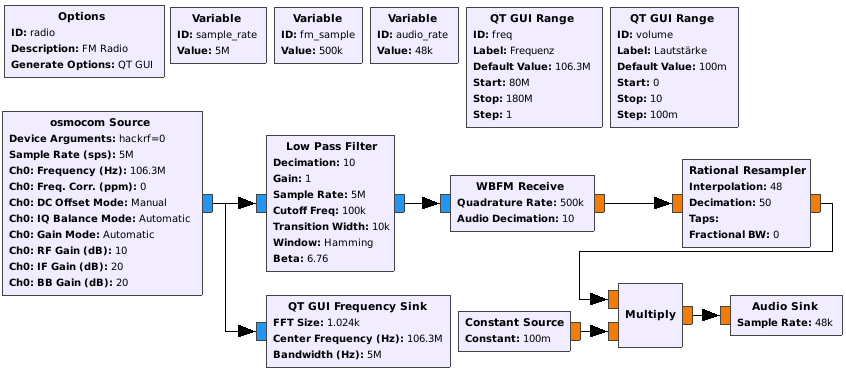
\includegraphics[width=\textwidth]{fmradio.png}
	\caption[Implementation eines FM-Radioempfängers in GNU Radio Companion]{Implementation eines FM-Radioempfängers in GNU Radio Companion. Quelle: Eigene Darstellung} 
	\label{fmradio}
\end{figure}

Das dargestellte Blockschaltbild realisiert das Empfangen, Demodulieren und Wiedergeben eines FM-Radio Signals. Das Programm bietet zudem die Möglichkeit Frequenz und Lautstärke anzupassen:

\begin{figure}[ht]
	\centering
	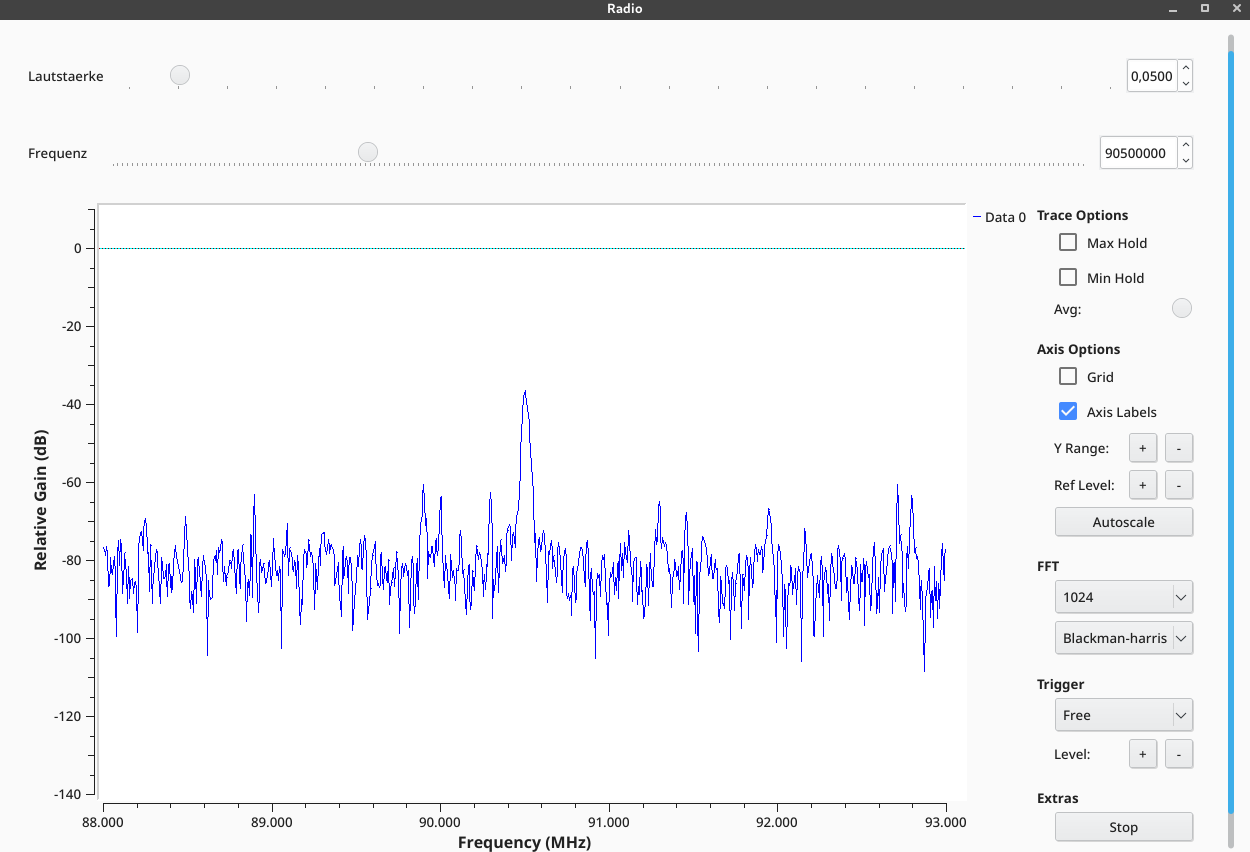
\includegraphics[width=0.8\textwidth]{fmradio-fft.png}
	\caption[FM Radio FFT-Plot]{FM Radio FFT-Plot. Quelle: Eigene Darstellung} 
	\label{fmradio-fft}
\end{figure}

Im Folgenden werden die einzelnen Bausteine näher erläutert.


\newpage
Als Signalquelle können in GNU Radio TCP/UDP Ports, Soundkarten, Dateien bzw. Input-Streams oder \ac{SDR}-Geräte benutzt werden.\newline
Um das HackRF One als Signalquelle zu verwenden, wird der quelloffene, von \ac{osmocom} \cite{osmocom:2018} entwickelte GNU Radio Block \textit{gr-osmosdr} \cite{gr-osmosdr:2018} benutzt.
Dieser untersützt das HackRF durch die zuvor installierte Bibliothek \textit{libhackrf}:

\begin{figure}[ht]
	\centering
	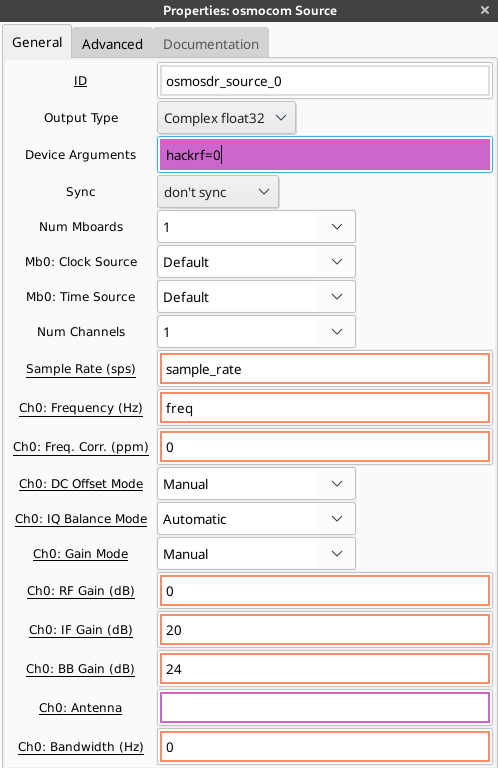
\includegraphics[width=0.5\textwidth]{osmocom-source.png}
	\caption[osmocom Source Block]{osmocom Source Block. Quelle: Eigene Darstellung} 
	\label{osmocom-source}
\end{figure}

\begin{description}
	\item[ID:] Der Name der Python-Variable des GRC Blocks. Variablennamen und Werte müssen mit denen der Python Spezifikation übereinstimmen, da diese beim Ausführen des Programmes in das entstehende Skript übernommen werden.
	\item[Output Type:] Der vom Block produzierte Datentyp, in diesem Fall \textit{Complex float32}, da das HackRF One Samples als IQ-Paare darstellt, wobei die I- und Q-Komponente jeweils als Float-Gleitkommazahl repräsentiert werden.
	\item[Device Arguments:] Dieser Wert identifiziert die zu verwendende Hardware. Da nur ein SDR Gerät bzw. HackRF angeschlossen ist, registriert dieses sich mit der ID 0. Alternativ kann das Gerät auch über dessen Seriennummer adressiert werden.
	\item [Sample Rate (sps):] Die Abtastrate $f_a$ in Samples pro Sekunde.
	\item[Ch0 Frequency (Hz):] Die Frequenz des Kanals. Da nur eine Antenne vorhanden ist, wird automatisch Channel 0 benutzt.
	\item[Ch0 Freq. Corr. (ppm):] Besonders bei RTL-SDR Geräten wie DVBT-Sticks, die keine hochwertigen Analog-Digital-Konverter nutzen, kommt es bei der Synchronisation ebendieser zu Abweichungen die in ppm (Parts per Million) angegeben und in Software korrigiert werden können \cite[vgl. Whiting, e. a., S.1]{ppm}.
	\item[Ch0 RF Gain (dB):] Die \ac{RF} Verstärker des HackRF One befinden sich nahe des Antennenanschlusses befinden, je einen für das Senden und Empfangen. Diese sind entweder ausgeschaltet oder verstärken mit 14 dB.
	\item[Ch0 IF Gain (dB):] \ac{IF} Gain regelt die Verstärkung der Zwischenfrequenz (bevor das Signal ins Basisband umgesetzt wird, überführt das HackRF es zur effizienteren Verarbeitung in eine Zwischenfrequenz). Es sind Werte von 0 - 40 dB möglich.
	\item[Ch0 BB Gain (dB):] Die Basisbandverstärkung des Signals. Erlaubt sind für das HackRF Werte zwischen 0 und 62 dB.
	\item[Ch0 Bandwidth (Hz):] Die zu verwendende Bandbreite hängt von dem zu betrachtenden Signal ab. 
\end{description}






\section{Erarbeiten der relevanten Metainformationen}
Maßgebend für das Erkennen und Verarbeiten von Signalen im Kontext von Software Defined Radio sind die Randbedingungen, gestellt von eingesetzter Hard- und Software, Umweltbedingungen und Signalarten.
Im folgenden wird eine Übersicht der relevanten Rahmenbedingungen und Kennzahlen, zusammengefasst im Begriff \enquote{Metainformationen} gegeben.
%TODO: Quantisierung / Diskretisierung

\subsection{Signalleistung}
\subsection{Modulation}
\subsection{DC Offset}
Durch die Überführung eines modulierten Signals zurück ins Basisband entsteht im FFT-Plot um die Nullfrequenz eine deutlich wahrnehmbare Spitze:
\begin{figure}[ht]
	\centering
	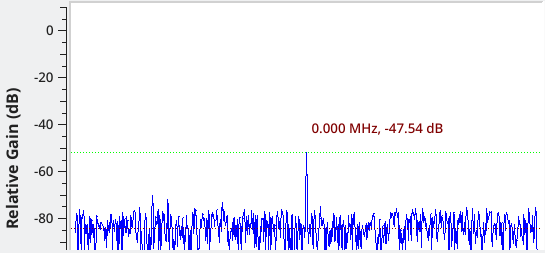
\includegraphics[width=0.6\textwidth]{dc-offset.png}
	\caption[DC Offset]{DC Offset. Quelle: Eigene Darstellung} 
	\label{dc-offset}
\end{figure}

Es gibt verschiedene Wege damit umzugehen:
\begin{enumerate}
	\item Für einige Anwendungen kann das DC Offset einfach vernachlässigt werden.
	\item Das DC Offset lässt sich für viele Signalarten umgehen indem die hohe Bandbreite des HackRF ausgenutzt wird. 
	Dazu stellt man nicht die Zielfrequenz ein, sondern eine außerhalb liegende Frequenz, so dass das eigentlich zu erfassende Signal von 0 Hz  weggeschoben wird. Weil das Signal natürlich vollständig in der erfassten Bandbreite enthalten sein muss, erhöht sich die Menge der zu analysierenden Daten und damit auch die CPU Auslastung. Die Bandbreite des SDR Gerätes sollte also bestenfalls nur so groß sein wie nötig um unnötige Last zu vermeiden.
	\item Das DC Offset lässt sich über Software korrigieren bzw. abschwächen. Das führt unter Umständen dazu dass auch Frequenzen nahe 0 Hz ungewollterweise modifiziert werden. Das Signal wird hierdurch also leicht verfälscht. Einige Spektralanalyseprogramme (GQRX, SDR\#) bieten dieses Feature an.
\end{enumerate}

\begin{figure}[ht]
	\centering
	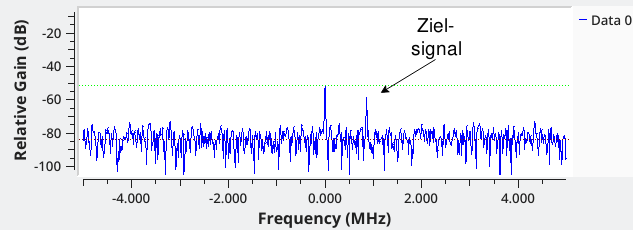
\includegraphics[width=0.7\textwidth]{dc-offset-correction.png}
	\caption[DC Offset Korrektur]{DC Offset Korrektur. Quelle: Eigene Darstellung} 
	\label{dc-offset-correction}
\end{figure}



\subsection{Empfängerempfindlichkeit}
\subsubsection{Signal-Rausch-Verhältnis}
Das Signal-Rausch-Verhältnis (engl.: \enquote{Signal-to-Noise Ratio}) gibt das Verhältnis eines Nutzsignals 
zu einem Rauschsignal an, von dem es überlagert ist. Das Rauschen kann dabei durch das Empfängersystem selbst, 
sowie durch Störungen im Übertragungskanal verursacht worden sein. %TODO: Es gibt glaub mehrere Definitionen

\[ S/N = \frac{\text{Nutzsignalleistung}}{\text{Rauschsignalleistung}} = \frac{P_{Signal}}{P_{Rauschen}} \]


Für den Fall \(P_{Signal} \leq P_{Rauschen}\), also wenn gilt: 
Die Signalleistung ist kleiner oder gleich der Rauschsignalleistung, kann ein Signal in der Regel nicht erkannt werden.
Damit dies gelingt, muss die Energie des Signals addiert mit der des Rauschsignals größer sein als ein festgelegter Schwellwert.
Der Schwellwert wird wesentlich höher gelegt, als das durchschnittliche Rauschniveau, um die beiden deutlich von einander unterscheiden zu können.
Es bietet sich also an das Verhältnis in Dezibel auszudrücken:
\[ S/N = 10 \lg \Big( \frac{P_{Signal}}{P_{Rauschen}} \Big) \text{dB}\] 



Das minimale Signal-Rausch-Verhältnis \(S/N_{min}\) gibt diesen Schwellwert an, der mindestens erreicht werden muss um das Signal zu erkennen. 
%TODO: Nutzsignalleistung und Rauschsignalleistung definieren

\subsection{Schlussfolgerung}
Viele Kennwerte von Signalen, dazu gehören auch das Signal-Rausch-Verhältnis oder die Signalleistung, sind stark abhängig von der verwendeten Hardware und Implementierung.
Die Frage danach, wie sich solche Kennzahlen bzw. Metainformationen allgemeingültig messen lassen, kann deshalb nicht eindeutig beantwortet werden.
Stattdessen wäre es besser eine spezifische Fragestellung zu formulieren, wie: \\
Was ist der minimale Leistungspegel eines Signales in dBm, mit der Modulationsart M auf der Frequenz F, welche von einem SDR-Gerät D mit Antenne A, unter Verwendung der Software S und Konfiguration K erkannt werden kann, mit einer maximalen Fehlerrate von E?\\
Die daraus resultierende Funktion mehrerer Variablen, \(P_{Signal} (M, F, D, A, S, K, E)\), kann Aufschluss darüber geben, ob etwa das HackRF One für einen bestimmten Einsatzzweck geeignet ist.

\newpage
\section{GRC-Flowgraph zur Analyse von Metadaten}
Aus den in diesem Kapitel behandelten Kennwerten wird im Folgenden ein GNU Radio Companion Programm erstellt, welches es erlaubt diese Informationen zu visualisieren. Zudem bietet die grafische Oberfläche diverse Einstellungsmöglichkeiten um Signale gemäß ihrer individuellen Eigenschaften angemessen betrachten zu können.

Die Einstellungsmöglichkeiten sind:

\begin{description}
	\item [Frequenz:] Angabe möglich in Schritten von 1 Hz. Das Frequenzspektrum ist begrenzt auf den Bereich der Dezimeterwelle. Der limitierende Faktor ist hier die Bandbreite der Antenne.
	\item [Abtastrate:] Angabe möglich in Schritten von 1 Hz. Die Sampling Rate ist begrenzt auf den Bereich von 0 Hz bis 20 MHz. Der limitierende Faktor ist hier die maximale Abtastrate des HackRF One.
	\item [DC Offset:]  Angabe möglich in Schritten von 1 Hz. Der Bereich ist begrenzt durch die maximale Bandbreite des HackRF One.
	\item[Bandbreite:] Angabe möglich in Schritten von 1 Hz. Die maximale Bandbreite beträgt 20 MHz. 
\end{description}

\begin{figure}[ht]
	\centering
	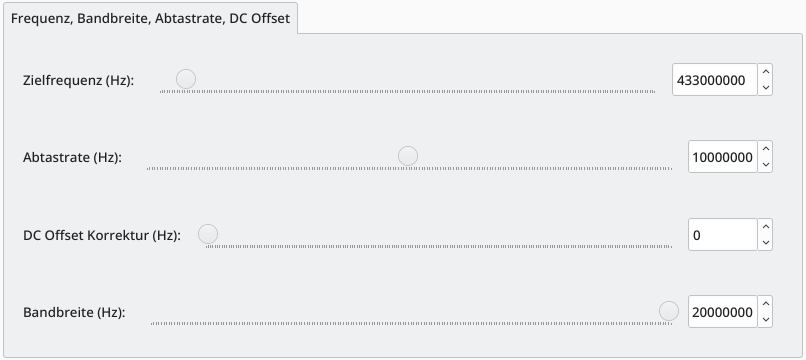
\includegraphics[width=\textwidth]{grc-freq.png}
	\caption[Frequenz, Bandbreite, Abtastrate, DC Offset]{Frequenz, Bandbreite, Abtastrate, DC Offset. Quelle: Eigene Darstellung, GNU Radio 3.7.11} 
	\label{grc-freq}
\end{figure}

\newpage
\begin{description}
	\item[RF Gain:] Entweder 0 dB, oder 14 dB. 
	\item[IF Gain:] Einstellbar in Schritten von 8 dB, im Bereich zwischen 0 und 40 dB.
	\item[BB Gain:] Einstellbar in Schritten von 2 dB, im Bereich zwischen 0 und 62 dB.
\end{description}

\begin{figure}[ht]
	\centering
	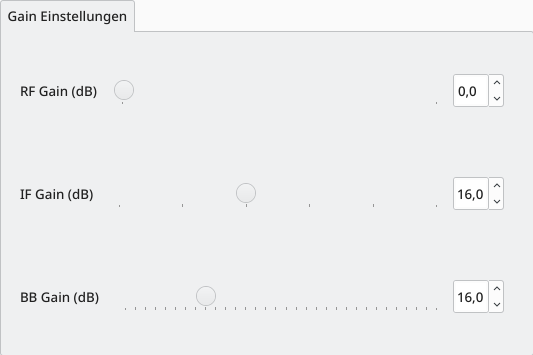
\includegraphics[width=0.65\textwidth]{grc-gain.png}
	\caption[Gain Einstellungen]{Gain Einstellungen. Quelle: Eigene Darstellung, GNU Radio 3.7.11} 
	\label{grc-gain}
\end{figure}

Die Visualisierung der Signale kann in den folgenden Darstellungen erfolgen:
\begin{description}
	\item[Frequenzdarstellung:] Als FFT-Plot. Es lassen sich einstellen:
		\begin{itemize}
			\item Max/Min Hold: Halten der maximalen bzw. minimalen Werte im Frequenzdiagramm.
			\item Anzeige der RF Frequenzen: Die Beschriftung der x-Achse kann entweder im Basisband erfolgen (Zentrierung um die Nullfrequenz), oder es werden die \enquote{tatsächlichen} Frequenzen (RF Frequencies) benutzt.
			\item  Averaging: Das Averaging ermöglicht eine Mittelung der aufgenommen Samples
			\item FFT Size: Steuert die Frequenzauflösung, also die Anzahl Abstufungen im FFT-Plot. Gemäß Abschnitt \ref{fft-grundlagen} muss der Wert einer Zweierpotenz entsprechen.
			\item Fensterfunktionen: Die von GNU Radio unterstützten Fensterfunktionen können hier ausgewählt werden.
		\end{itemize}
	\item[Wasserfalldiagramm:] GNU Radio ermöglicht die Darstellung von Signalen auch als Wasserfalldiagramm. Die Schwellwerte der Farbintensitäten können hier eingestellt werden. 
	\item[Zeitdomäne:] Hier können Signale als im Zeitbereich betrachtet werden.
	\item[Konstellationsdarstellung] (engl.: \enquote{Constellation Display}): Hierdurch wird die Betrachtung der Ortskurven empfangener I/Q-Daten ermöglicht.
\end{description}

\begin{figure}[ht]
	\centering
	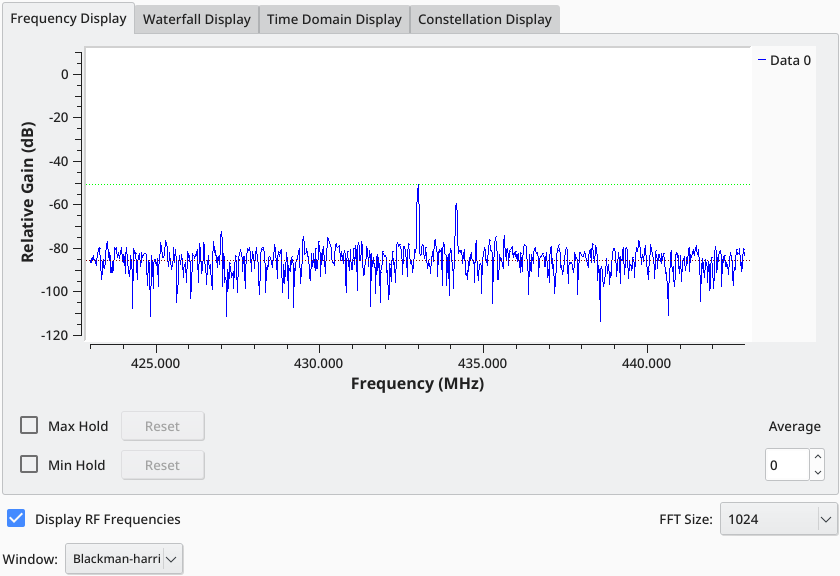
\includegraphics[width=0.8\textwidth]{grc-qt-gui.png}
	\caption[Darstellung im Frequenzbereich]{Darstellung im Frequenzbereich. Quelle: Eigene Darstellung, GNU Radio 3.7.11} 
	\label{grc-qt-gui}
\end{figure}



Das resultierende Programm als GRC Flowgraph wird in der folgenden Grafik dargestellt:
\begin{figure}[H]
	\centering
	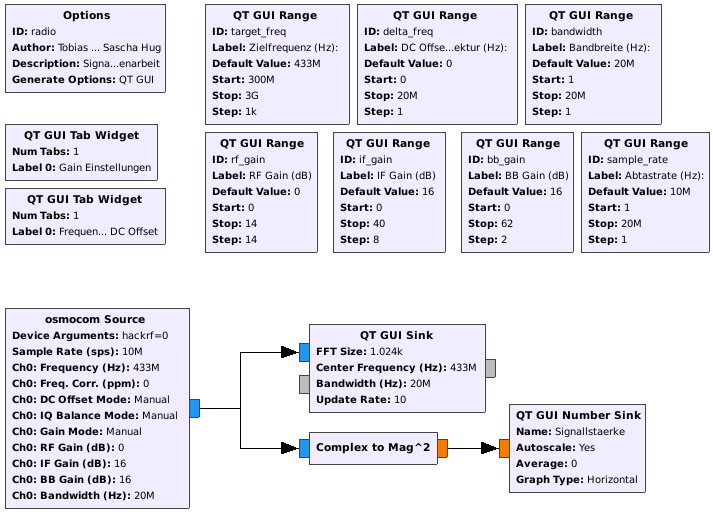
\includegraphics[width=0.85\textwidth]{grc-flowgraph.png}
	\caption[GRC Flowgraph zur Metaanalyse]{GRC Flowgraph zur Metaanalyse. Quelle: Eigene Darstellung, GNU Radio 3.7.11} 
	\label{grc-flowgraph}
\end{figure}

\section{Identifizieren und Dekodieren eines Signales}
Signale müssen im Empfänger gemittelt werden, da sie aufgrund der durchgeführten Kanalfilterung ein oszillierendes Verhalten aufweisen, siehe Abb. \ref{mod-send-empf} \cite[vgl. Heuberger, e. a., S. TODO]{Heuberger:2017}.

\begin{figure}[ht]
	\centering
	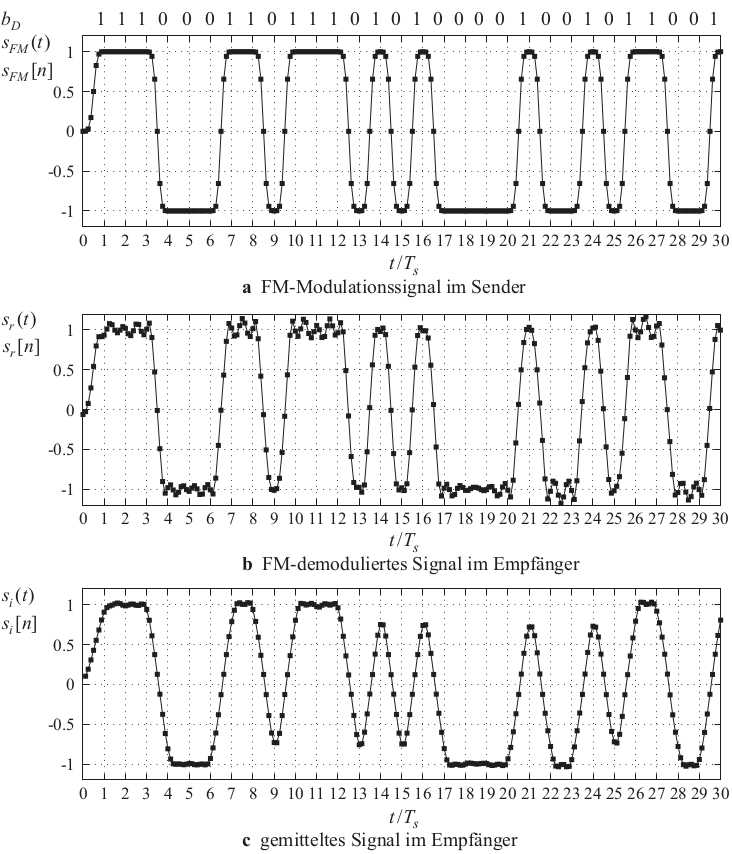
\includegraphics[width=0.8\textwidth]{mod-sender-empf.png}
	\caption[GFSK-Modulationssignale im Sender und im Empfänger]{GFSK-Modulationssignale im Sender und im Empfänger. Quelle: TODO} %TODO Selbst darstellen, am besten anhand eines 433MHz Signals! 
	\label{mod-send-empf}
\end{figure}


\newpage
